\documentclass[a4paper]{report}
    
    \usepackage[english]{babel}
    \usepackage[utf8]{inputenc}
    \usepackage{amsmath}
    \usepackage{graphicx}
    \usepackage[colorinlistoftodos]{todonotes}



    % CUSTOM MARGIN AND PARAMETER
    \usepackage[a4paper, portrait, left=1.2in,right=1in,bottom=1in,top=1in]{geometry}

    \usepackage{sectsty}
    
    \sectionfont{\fontsize{12pt}{0}\selectfont}
    \subsectionfont{\normalfont \itshape \fontsize{12pt}{0}\selectfont}
    \subsubsectionfont{\normalfont \itshape \fontsize{12pt}{0}\selectfont}
    \paragraphfont{\fontsize{12pt}{0}\selectfont}
    \chapterfont{\fontsize{14pt}{0}\selectfont}

		

    \title{Quantum Hall effect report template}   

    \title{Backend and Analytics as a service}
    
    \author{Aditya and Shubham}
    
    \date{\today}
    
    \begin{document}
    
    \begin{titlepage}
      \maketitle 
    \end{titlepage}    
    
    \newpage
    \tableofcontents{}    

    \chapter {Introduction}
    
    \section{Preamble}
    \label{sec:introduction}    
    Explain the context of the experiment here. Why is condensed matter physics interesting or important?
    Optional things you could talk about (but don't have to -- this is up to you): transistors, computers, Quantum computers, fundamental knowledge (e.g. the resistance quantum).    
    Briefly explain what methods you will use in the experiment, and what values you will extract from the data.    
    For this section and all following sections: If you refer to an equation, previous result or theory that is not regarded as common knowledge, then cite the source (article or book) where you found this. For example, you can cite the Nano 3 Lecture notes \cite{nano3}.
    
    \section{Need of the project}
    \label{sec:theory}
    Here, explain the concept of a 2-DEG in GaAs/AlGaAs. What is a 2-DEG and why does it arise?
    \section{Problem Statement}
    Here, explain the concept of a 2-DEG in GaAs/AlGaAs. What is a 2-DEG and why does it arise?
    \section{Objectives}
    Explain the classical Hall effect in your own words. What do I measure at $B=0$? And what happens if $B>0$? Which effect gives rise to the voltage drop in the vertical direction?
    \section{Solution Approach}
    Explain the IQHE in your own words. What does the density of states look like in a 2-DEG when $B=0$? What are Landau levels and how do they arise? What are edge states? What does the electron transport look like when you change the magnetic field? What do you expect to measure?    
    \section{Organisation of the Project Report}    
    Explain a step-by-step recipe for fabrication here. How long did you etch and why? What is an Ohmic contact?
    
    
    \chapter {Background}
    Explain the experimental set-up here. Use a schematic picture (make it yourself in photoshop, paint, ...) to show how the components are connected. Briefly explain how a lock-in amplifier works.
    
    \section{Area,available tools and hardware and software}
    Show a graph of the longitudinal resistivity ($\rho_{xx}$) and Hall resistivity ($\rho_{xy}$) versus magnetic field, extracted from the raw data shown in figure \ref{fig:data}. You will have the link to the data in your absalon messages, if not e-mail Guen (guen@nbi.dk). Explain how you calculated these values, and refer to the theory.
    
    \begin{figure}
    \centering
    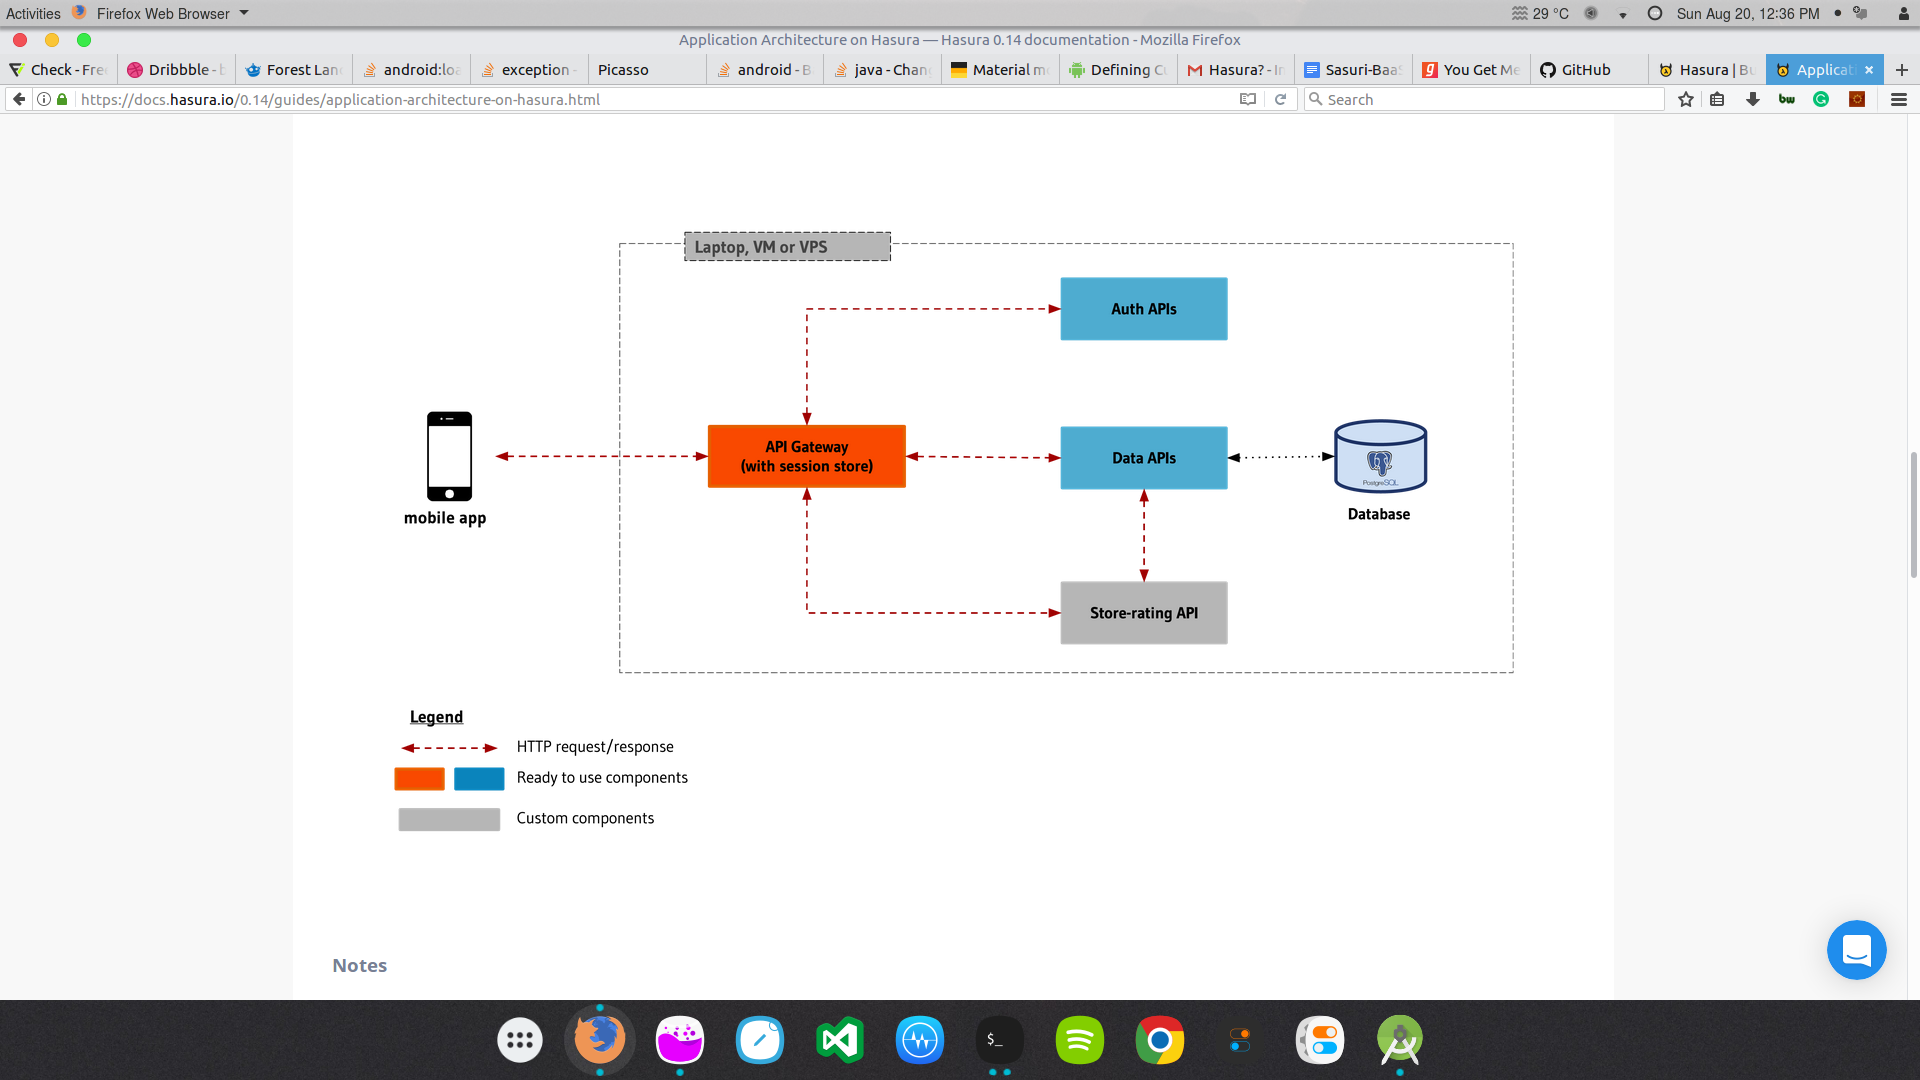
\includegraphics[width=1\textwidth]{test.png}
    \caption{\label{fig:data} Activity Diagram sample}
    \end{figure}
    
    \section{Literature review}
    Calculate the sheet electron density $n_{s}$ and electron mobility $\mu$ from the data in the low-field regime, and refer to the theory in section \ref{sec:theory}. Explain how you retrieved the values from the data (did you use a linear fit?).
    Round values off to 1 or 2 significant digits: 8.1643 ~= 8.2. Also, 5e-6 is easier to read than 0.000005.
    
    !OBS: This part is optional (only if you have time left).
    Calculate the uncertainty as follows: \newline $u(f(x, y, z)) = \sqrt{(\frac{\delta f}{\delta{x}} u(x))^{2} + (\frac{\delta f}{\delta{y}} u(y))^{2} + (\frac{\delta f}{\delta{z}} u(z))^{2}}$, where $f$ is the calculated value ($n_{s}$ or $\mu$), $x, y, z$ are the variables taken from the measurement and $u(x)$ is the uncertainty in x (and so on).
    
    \subsection{Area,available tools and hardware and software}
    Calculate $n_{s}$ for the high-field regime.
    Show a graph of the longitudinal conductivity ($\rho_{xx}$) and Hall conductivity($\rho_{xy}$) \textbf{in units of the resistance quantum} ($\frac{h}{e^{2}}$), depicting the integer filling factors for each plateau.
    Show a graph of the plateau number versus its corresponding value of $1/B$. From this you can determine the slope, which you use to calculate the electron density.
    Again, calculate the uncertainty for your obtained values.
    
    \subsection{Literature review}
    Discuss your results. Compare the two values of $n_{s}$ that you've found in the previous section. Compare your results with literature and comment on the difference. If you didn't know the value of the resistance quantum, would you be able to deduce it from your measurements? If yes/no, why?
    
    \chapter {Analysis}
    \section{Detailed Problem statement}
    \label{sec:theory}
    Here, explain the concept of a 2-DEG in GaAs/AlGaAs. What is a 2-DEG and why does it arise?
    \section{Requirement Analysis}
    Here, explain the concept of a 2-DEG in GaAs/AlGaAs. What is a 2-DEG and why does it arise?
    \subsection{Functional Requirement}
    Explain the classical Hall effect in your own words. What do I measure at $B=0$? And what happens if $B>0$? Which effect gives rise to the voltage drop in the vertical direction?
    \subsection{Non-Functional Requirement}
    Explain the IQHE in your own words. What does the density of states look like in a 2-DEG when $B=0$? What are Landau levels and how do they arise? What are edge states? What does the electron transport look like when you change the magnetic field? What do you expect to measure?    
    \section{Feasibility Study}    
    Explain a step-by-step recipe for fabrication here. How long did you etch and why? What is an Ohmic contact?
    \section{Diagram (as per our project problem)}
    a
    \begin{figure}
    \centering
    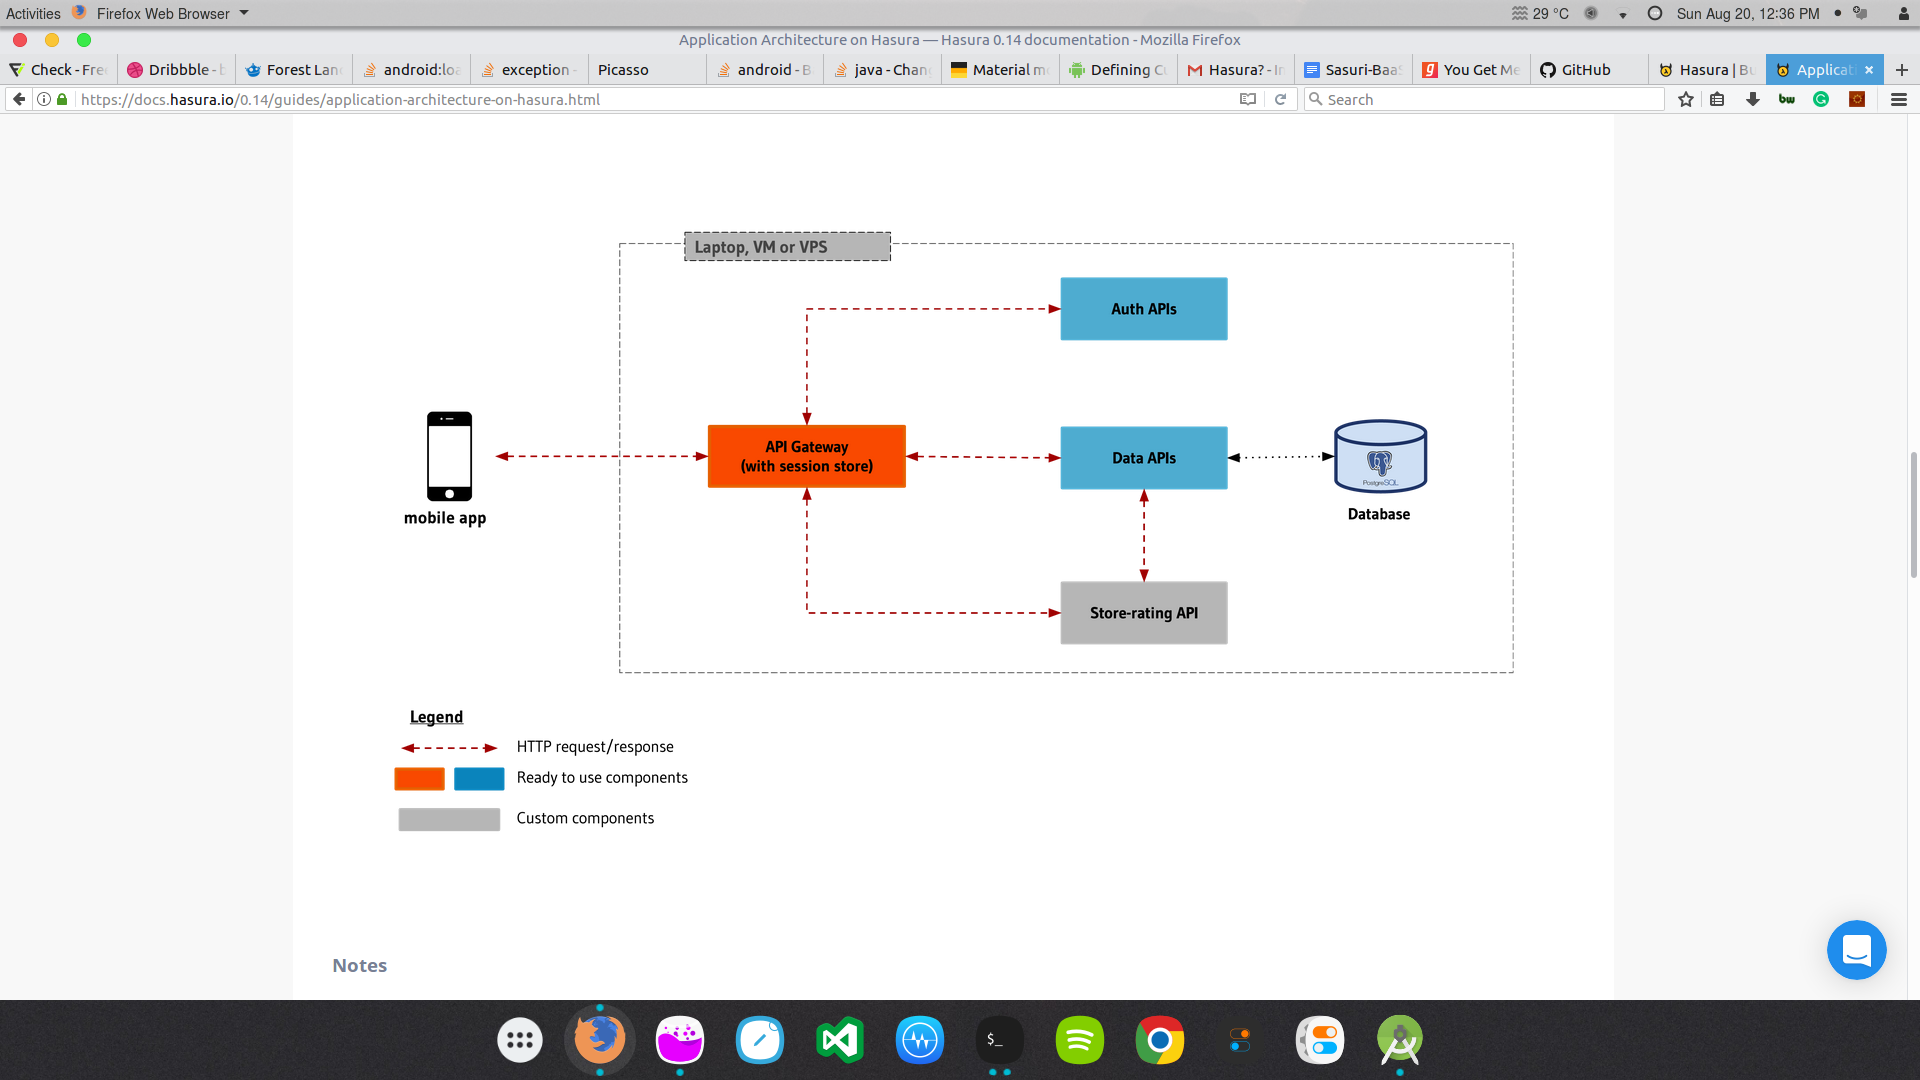
\includegraphics[width=1\textwidth]{test.png}
    \caption{\label{fig:data}Raw (unprocessed) data. Replace this figure with the one you've made, that shows the resistivity.}
    \end{figure}    
    
    \chapter {Architectural Diagrams}
    \section{Architectural Diagram. Discussion of moules}
    Architectural Designs
    \section{Algorithm Designed}
    Algorithm 
    \section{Diagrams}
    Diagrams

    \chapter {Conclusion}
    \section{Work carried out in phase 1}
    Architectural Designs
    \section{Work to be carried out in phase 2}
    Algorithm     


    \chapter{Sample items}
    \section{Some LaTeX tips}
    \label{sec:latex}
    \subsection{How to Include Figures}    
    First you have to upload the image file (JPEG, PNG or PDF) from your computer to writeLaTeX using the upload link the project menu. Then use the includegraphics command to include it in your document. Use the figure environment and the caption command to add a number and a caption to your figure. See the code for Figure \ref{fig:frog} in this section for an example.            
    \subsection{How to Make Tables}    
    Use the table and tabular commands for basic tables --- see Table~\ref{tab:widgets}, for example.    
    \begin{table}
    \centering
    \begin{tabular}{l|r}
    Item & Quantity \\\hline
    Widgets & 42 \\
    Gadgets & 13
    \end{tabular}
    \caption{\label{tab:widgets}An example table.}
    \end{table}    
    \subsection{How to Make Sections and Subsections}
    
    Use section and subsection commands to organize your document. \LaTeX{} handles all the formatting and numbering automatically. Use ref and label commands for cross-references.
    
    \subsection{How to Make Lists}
    
    You can make lists with automatic numbering \dots
    
    \begin{enumerate}
    \item Like this,
    \item and like this.
    \end{enumerate}
    \dots or bullet points \dots
    \begin{itemize}
    \item Like this,
    \item and like this.
    \end{itemize}
    \dots or with words and descriptions \dots
    \begin{description}
    \item[Word] Definition
    \item[Concept] Explanation
    \item[Idea] Text
    \end{description}
    
    We hope you find write\LaTeX\ useful, and please let us know if you have any feedback using the help menu above.

    

    \begin{thebibliography}{9}
    \bibitem{nano3}
    	Francis Gropengießer and Kai-Uwe Sattler,
      \emph{Database Backend as a Service: Automatic Generation, Deployment, and Management of Database Backends for Mobile Applications}.
			Available at \underline{https://link.springer.com/article/10.1007/s13222-014-0157-y}
			
		\bibitem{nano3}
    	Francis Gropengießer and Kai-Uwe Sattler,
      \emph{Overview Of Backend as a Service (BaaS) White Paper}.
			Available at \underline{http://baas.apievangelist.com/2013/05/08/overview-of-backend-as-a-service-baas-white-paper/}
			
								
		\bibitem{nano3}
			Balkan, A. 2012,
      \emph{What are the pros and cons of using a backend as a service?}.
			Available at \underline{https://www.quora.com/What-are-the-pros-and-cons-of-using-a-backend-as-a-service}			
		
		\bibitem{nano3}
			Backend as a Service (BaaS) Market Global forecast for 2020,
			Available at \underline{http://www.marketsandmarkets.com/PressReleases/baas.asp}		
		
		\bibitem{nano3}
			Backendless website 2016,
      \emph{Database Backend as a Service: Automatic Generation, Deployment, and Management of Database Backends for Mobile Applications}.
			Available at \underline{https://backendless.com/what-is-backend-as-a-service/}
	

		\bibitem{nano3}
			Ryan Goodrich,
      \emph{What is BaaS (Backend as a Service)}.
			Available at \underline{http://www.businessnewsdaily.com/4992-what-is-baas.html}	
			
		\bibitem{nano3}
			Nguyen, T, 2016,
      \emph{Mobile Backend as a Service: The Pros and Cons of Parse
			Case company: SuperApp Oy}.
			Available at \underline{http://theseus.fi/bitstream/handle/10024/117483/Nguyen{\_}Phu.pdf?sequence=2}
		
		\end{thebibliography}	
    \end{document}